\subsection{$\qqh$ Event Seleciton} 
The $\qqh$ channel refers to $ZH$ production in which both $Z$ and Higgs bosons decays hadronically.
We require exclusively 4 jets reconstructed by Durham-like algorithm\cite{Durham} in final states, corresponding to the leading logrithm approximation of 4-partners final states. The domiant SM backgrounds are consist of diboson production followed by hadronic decays of both bosons, and quark pair production. Events with loosened isolation lepton candidates were rejected.
All of the 4 jets are required to contain at least 10 PFOs to remove the 
events with fake jets. 
The visible energy of each event are required to be larger than 206 \GeV 
to reject the events with energetic nuetrinos. 
In figure \ref{fig:VisEn_nPFO} visible energy and minimum PFO multicplicity of the jets distributions of signal and backgrounds are presented.\par
\begin{figure}
\label{fig:VisEn_nPFO}
\centering
\subfigure[]
{
  \begin{minipage}[b]{0.42\textwidth}
  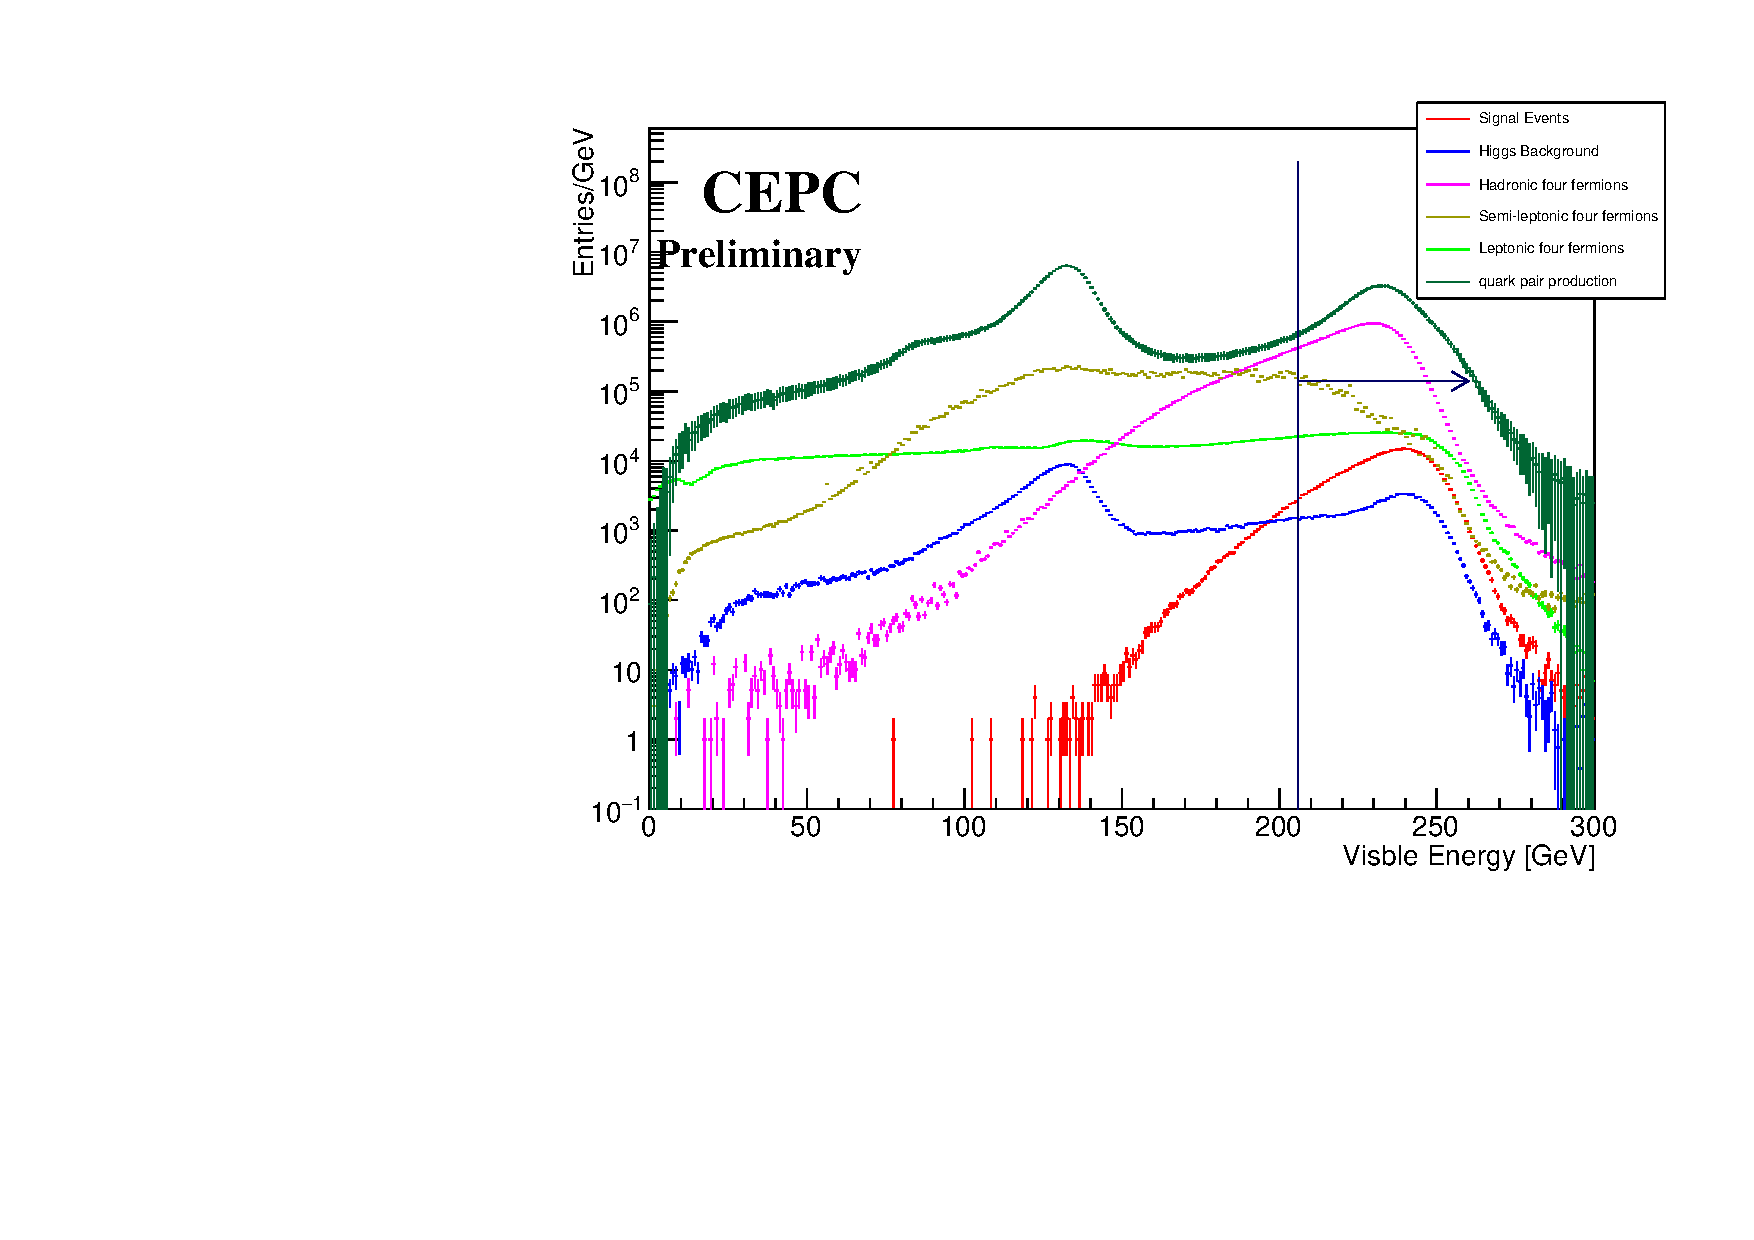
\includegraphics[width=\textwidth]{Analysis/qqh/VisEn.pdf}
  \end{minipage}
}
\subfigure[]
{
  \begin{minipage}[b]{0.42\textwidth}
  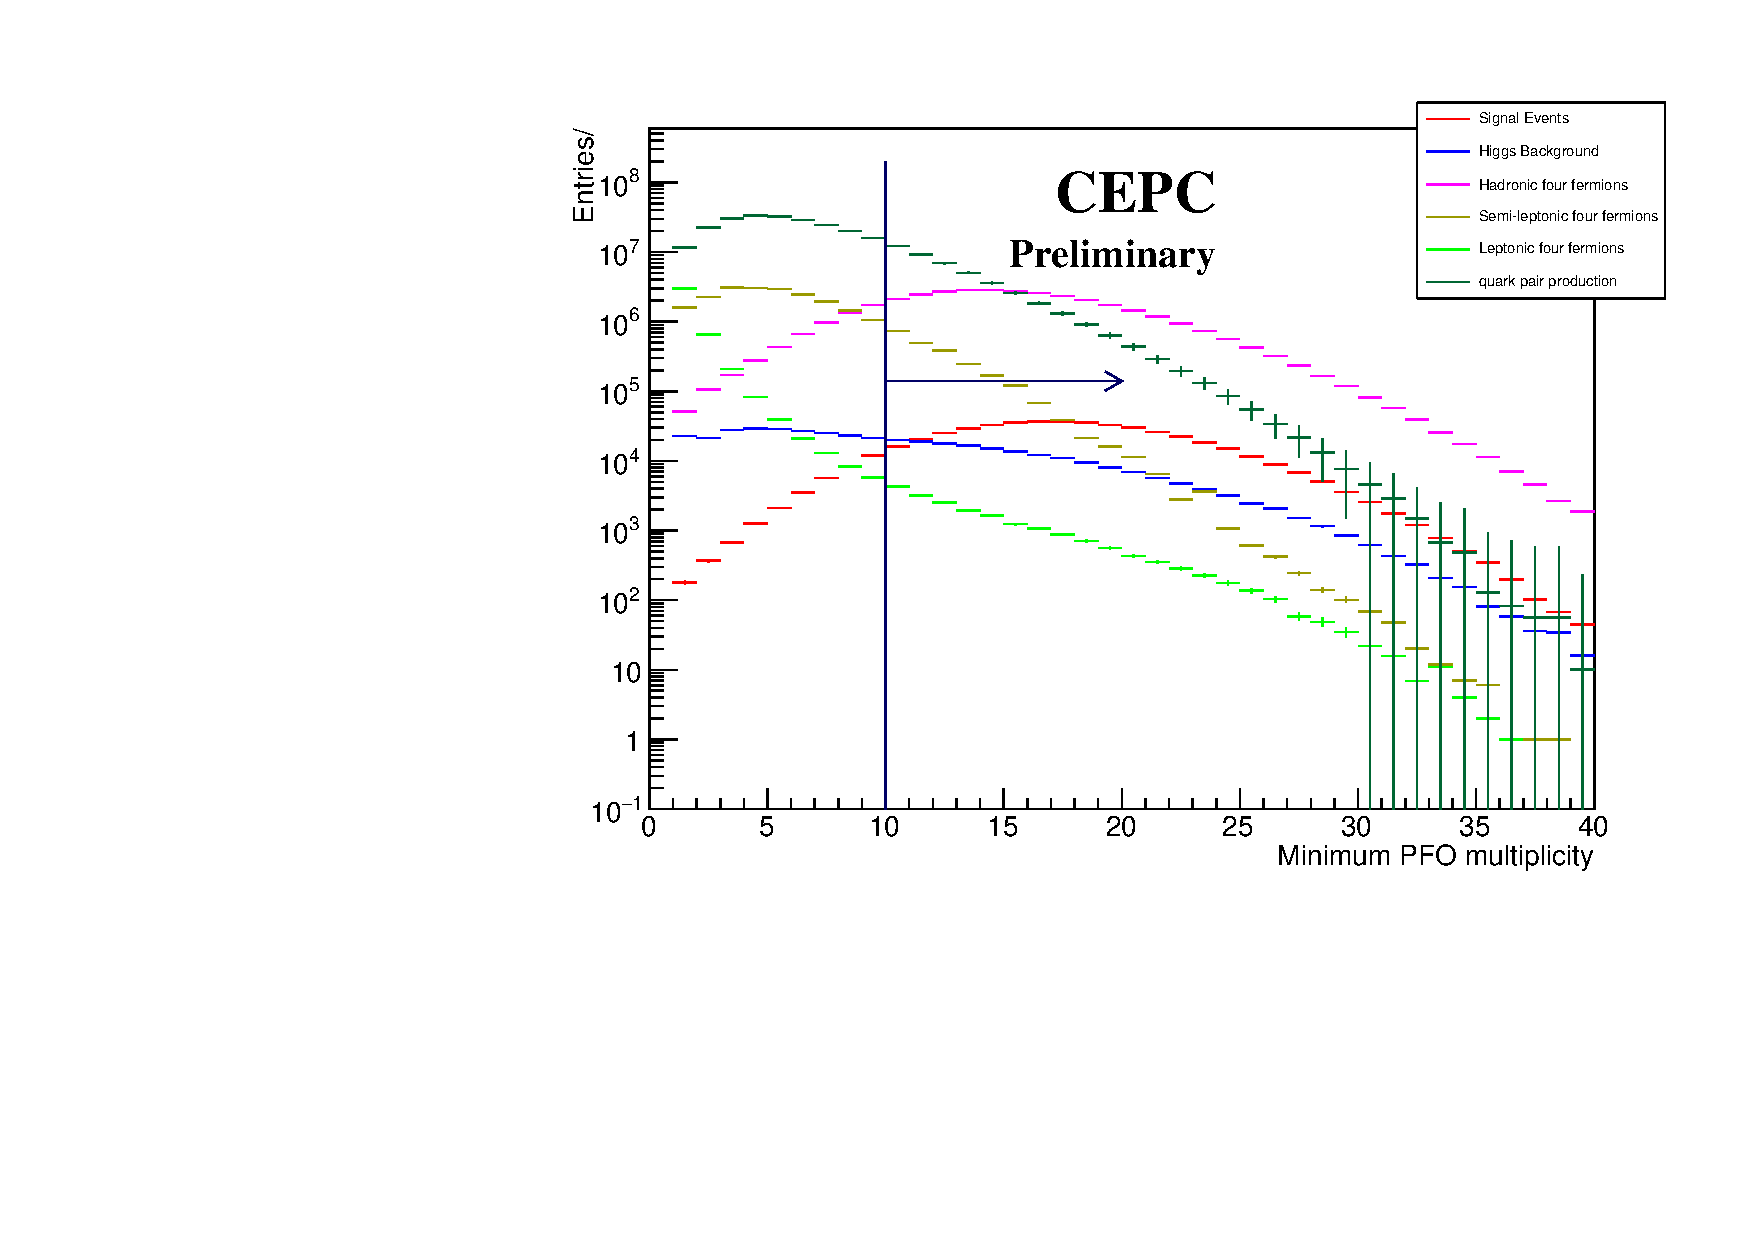
\includegraphics[width=\textwidth]{Analysis/qqh/nPFOmin.pdf}
  \end{minipage}
}
\caption{Distribution of visible energy(left) and minimum jets' pfo multiplicity(right) for the signal and SM backgrounds.}
\end{figure}


%It can also effectively remove the 2 fermions events with radiation return, since emitted photon can be missed from detection.

%To further suppress the background from 2 jets events, two variable are used as discriminator. One is called yth-value('th' refer to 3 and 4 here) which is constructed from PFO distributionthe other one is called sphericity, which represents the PFO distribution shape in each event. The distribution of \emiss, $y_34$ and sphericity can be found in figure \ref{fig:missingE}.
To suppress the background from 2 jets events, the $y_{34}$ are used as discriminator, which can effectively select the 4 jets events 
from those with lower jet multiplicity. A cut on the energetic-weighted angular 
dispersion was defined as $\Delta\theta$ variable, 
which was used in ALEPH 4-bjets channel analysis\cite{ALEPH_ZH_PLB}, is also used to furuther suppress the $q\bar{q}$ and semi-leptonic 4 fermions backgrounds.
 . The distribution of $y_{34}$ and $\Delta\theta$ can be found in figure 
 \ref{fig:y34_Deltatheta}.
 \begin{figure}
\label{fig:y34_Deltatheta}
\centering
\subfigure[]
{
  \begin{minipage}[b]{0.42\textwidth}
  \includegraphics[width=\textwidth]{Analysis/qqh/y34.pdf}
  \end{minipage}
}
\subfigure[]
{
  \begin{minipage}[b]{0.42\textwidth}
  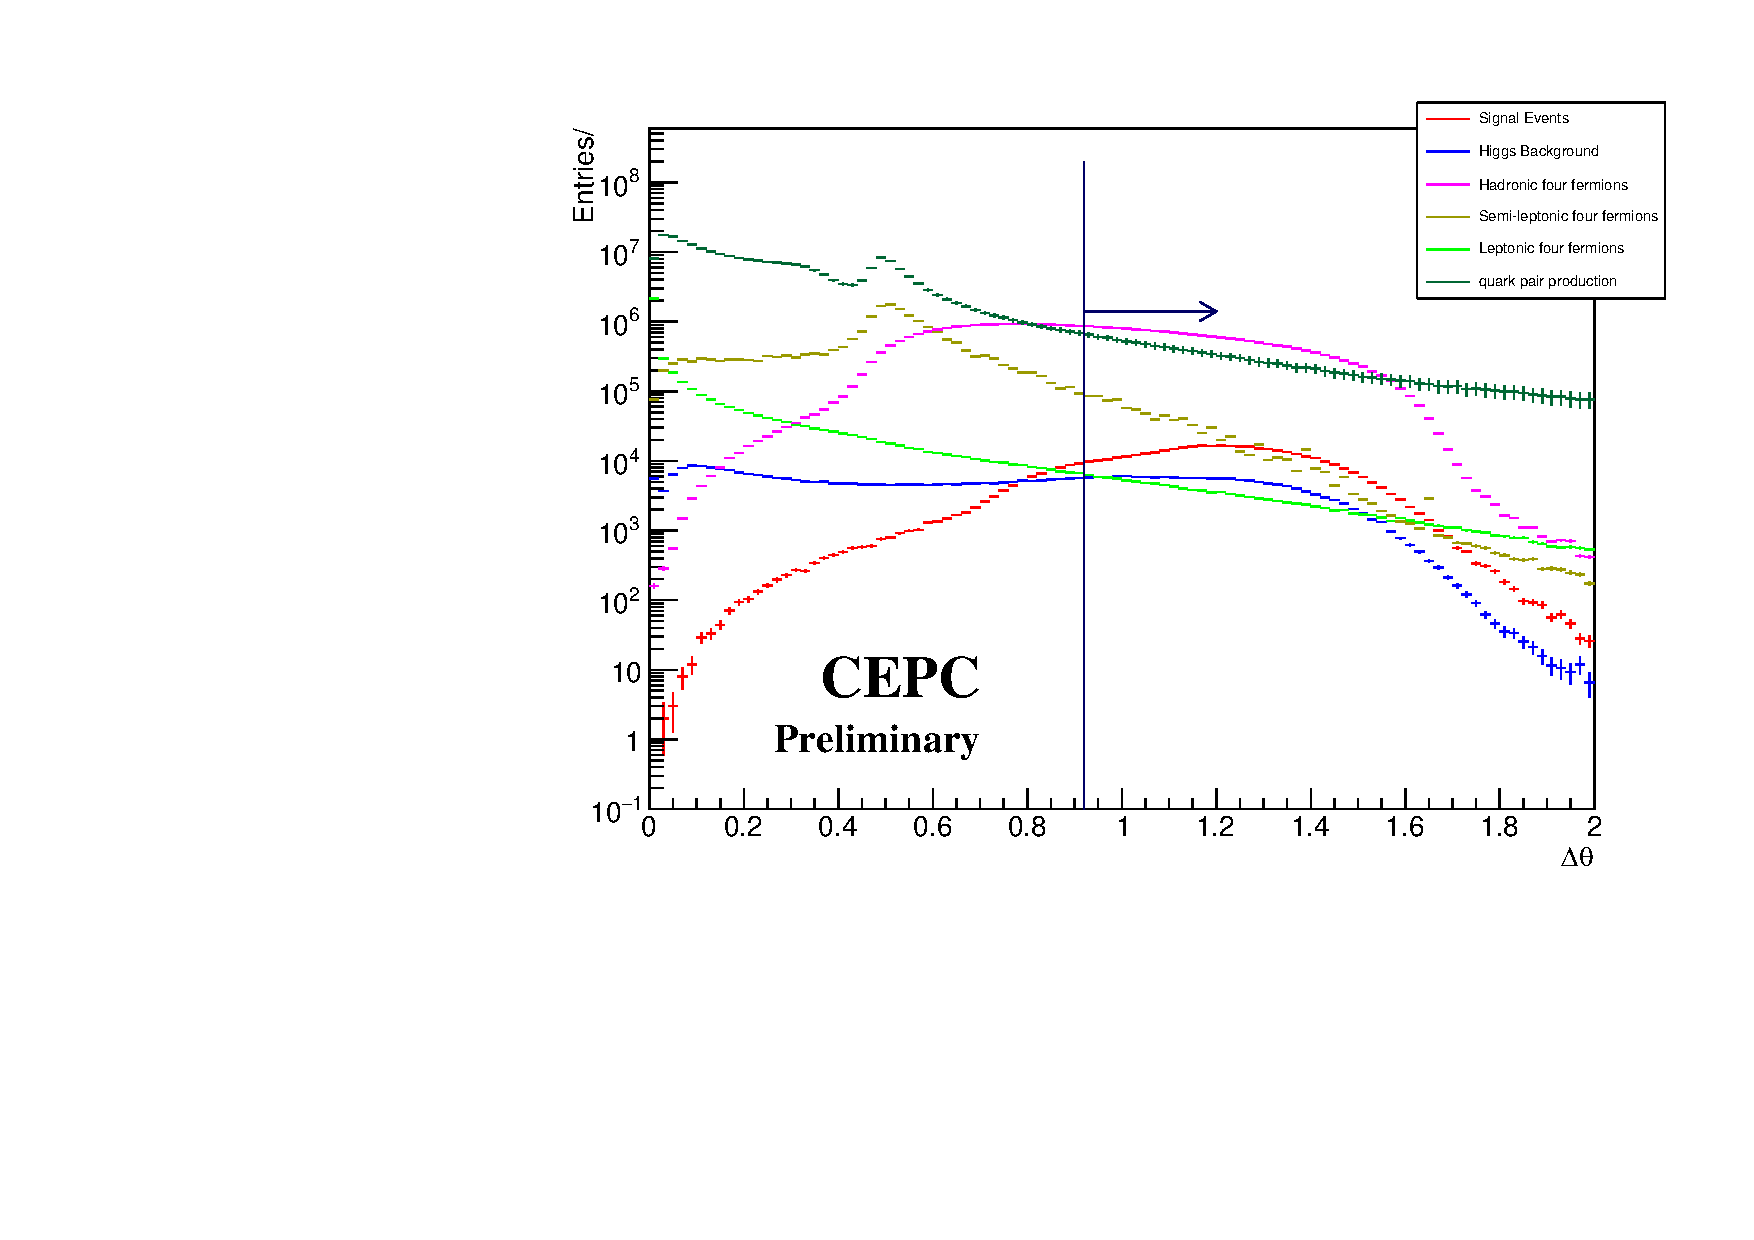
\includegraphics[width=\textwidth]{Analysis/qqh/DeltaTheta.pdf}
  \end{minipage}
}
\caption{Distribution of $y_{34}$(left) and $\Delta\theta$ (right) for the signal and SM backgrounds.}
\end{figure}
 \par 
%\begin{figure}[htpb]
%\centering
%    \includegraphics[width=0.45\textwidth]{figures/MissingE.pdf}
%    \includegraphics[width=0.45\textwidth]{figures/y34.pdf}
%    \includegraphics[width=0.45\textwidth]{figures/Sphericity.pdf}
%\caption{Distribution of MissingE, $y_{34}$ and sphericity of signal and background events, normalized to 5000 fb$^{-1}$
%}
%\label{fig:missingE}
%\end{figure}

The 4 jets in the final states are paired in order to get minimum $\chi^2$ defined as:
\begin{equation}
     \chi^2_{HZ} = \mathrm{min}\{(m_{ij}-m_H)/\sigma^2_{H} + (m_{kl}-m_Z)/\sigma^2_{Z} \}
     \label{for:chi2}
\end{equation}
in which i,j,k,l are the jet index, running from 1-4; $m_{ij}$ is the invariant mass of one jet pair and $m_{kl}$ is that of another pair; $m_H$ and $m_Z$ are Higgs and Z boson mass; $\sigma_H$ and $\sigma_Z$ are the width of reconstructed jet pair invariant mass from Higgs and  $Z$ boson. A variable $\chi^2_{WW}$ is defined in the similar way as formula \ref{for:chi2}, in which the $Z$/Higgs masses and widths are replaced by those of $W$ boson. The $\chi^2_{HZ}$ and $\chi^2_{ZZ}$ are combined into a variable $X$:
\begin{equation}
  X = \dfrac{\chi^2_{WW}-\chi^2_{HZ}}{chi^2_{WW}+\chi^2_{HZ}}
  \label{for:X}
\end{equation}
 The X value distrutes in the range from -1 to 1. For signal events, it tends to be positive 
 values(close to 1) while for the dominant $WW$ hadronic background, the X value tends to be negative(close to -1), as shown in figure \ref{fig:X}. Thus X provides discrimination power against $WW$ hadronic events.
 \begin{figure}
 \label{fig:X}
 \centering
 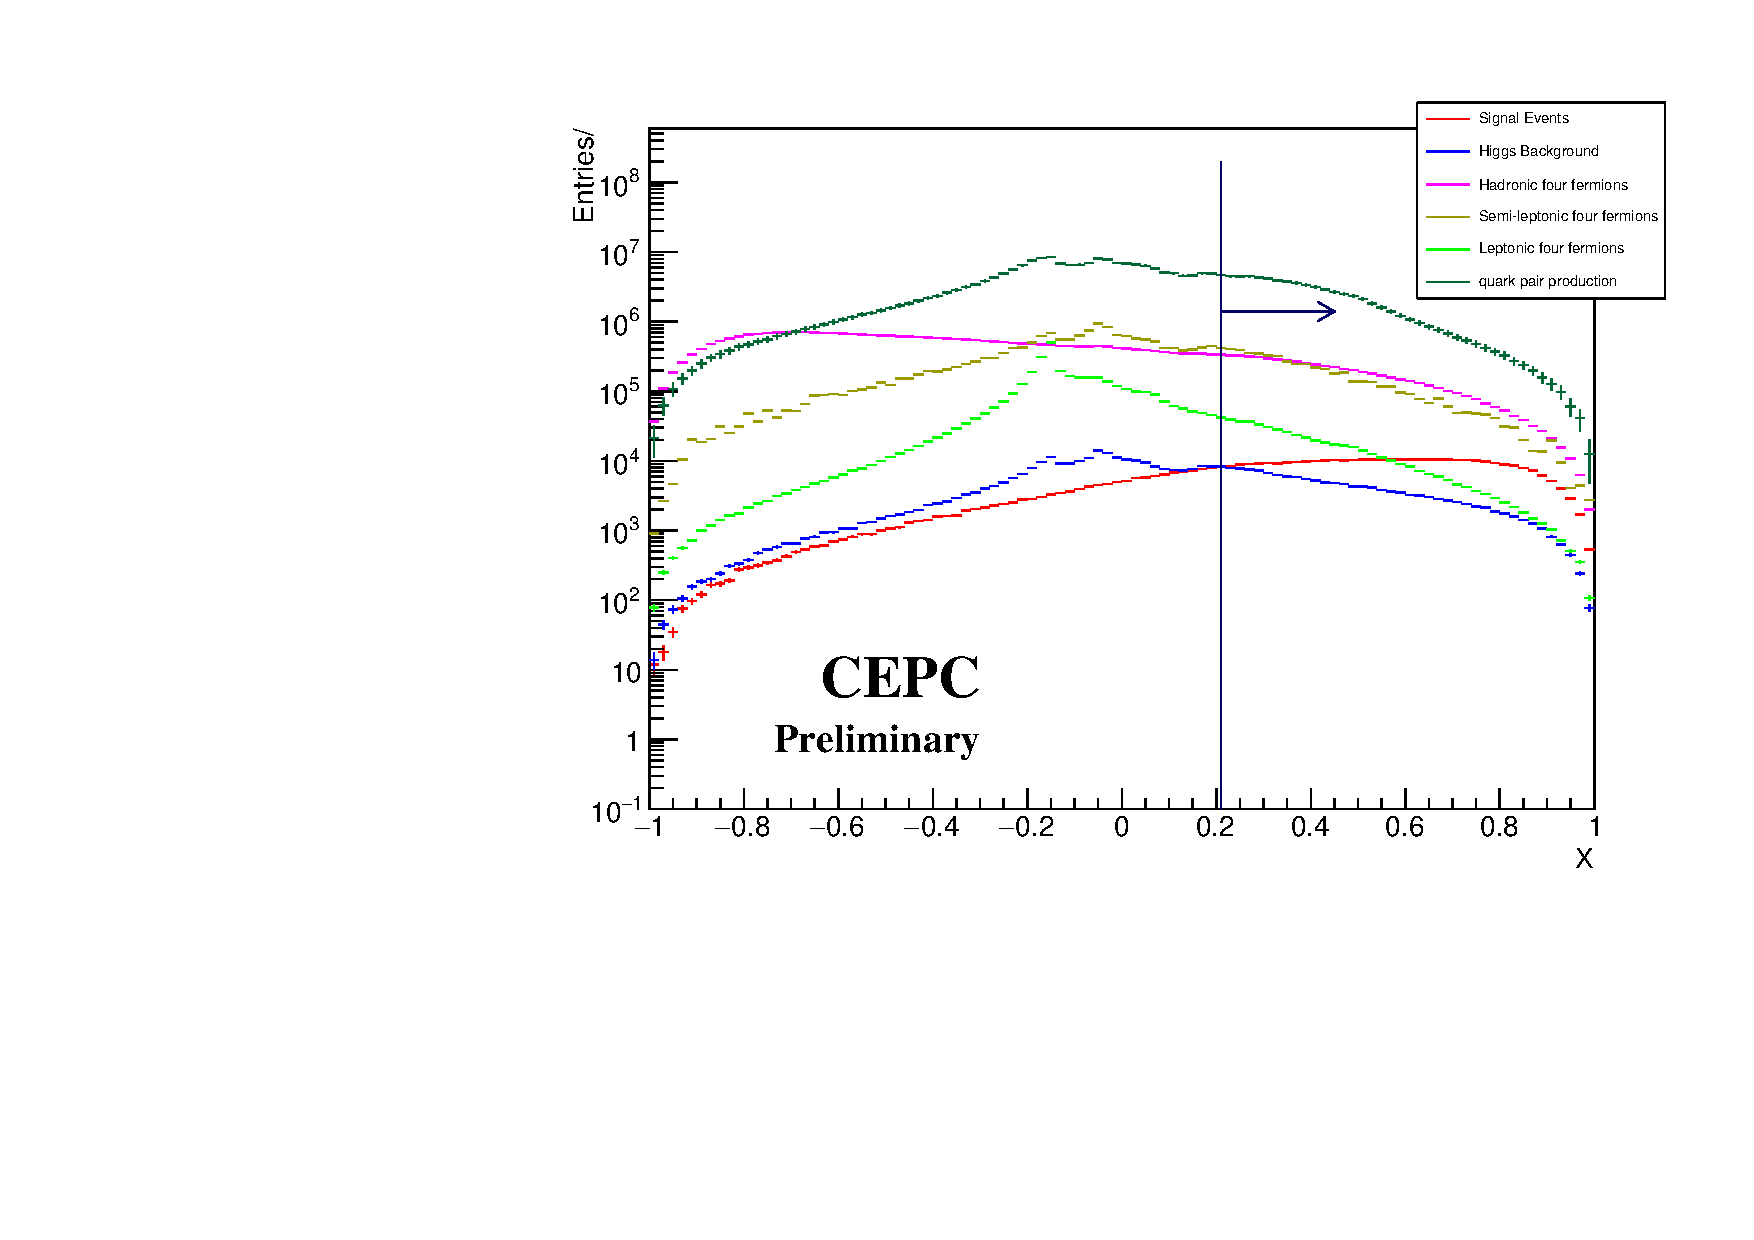
\includegraphics[width=0.67\textwidth]{Analysis/qqh/X.pdf}
 \caption{The distribution of $X$ defined in formula \ref{for:X}.}
 \end{figure}
\par
%invariant mass distribution of 2 jets from Higgs or Z correspondingly.  The distribution of 2 jet pair invariant mass can be found in figure \ref{fig:jet_pair_invmass}
%\begin{figure}[htpb]
%\centering
%    \includegraphics[width=0.45\textwidth]{figures/HZ_signal.eps}
%    \includegraphics[width=0.45\textwidth]{figures/HZ_4q.eps}
%\caption{Distribution of invariant mass of the two jet pairs for signal(left) and WW(right) events. The x-axis represents the invariant mass of a jet pair which is cloest to the higgs among all combination; the y-axis represents the invariant mass of another jet pair.
%}
%\label{fig:jet_pair_invmass}
%\end{figure}

%The results of the cutflow are summerized in table \ref{tab:cutflow}.
%\begin{table}[!htbp]
%\centering
%\begin{tabular}{|c|c|c|c|c|c|c|c|c|c|} \hline
%         &   signal   & other qqH      &  ffH   &  qq   &  ll   &  qqqq  &   llqq   &  lvqq   & vvqq  leptonic \\ \hline
%Dataset  &  \multicolumn{2}{c|}{724k}  &  405k  & 250M  & 20.4M & 36.9M  &  3.2M    &  36.45M &  2.17M    \\ \hline
%  4J FS  &  494.6k    &   214.2k       & 299.4k &\multicolumn{2}{c|}{267.1M}
%                                                                & 36.85M &  3.16M   &  35.9 M & 1.36M   \\ \hline
%  Iso Lep Veto
%         & 489.7k     &   154.4k       & 130.9k &\multicolumn{2}{c|}{242.2M}
%                                                                & 36.2M  & 558.4k   &  9.33M  & 1.35M     
%                                                                \\ \hline
%  \emiss$<$76 GeV
%         & 487.3k     &   130.2k       & 15.9k  &\multicolumn{2}{c|}{238.8M}
%                                                                & 36.11M & 354.5k   &  3.1M   & 964         \\ \hline
%  $y_{34}>$0.013
%        & 339.1k     &  99.34k        & 8.71k  &\multicolumn{2}{c|}{12.58M}
%                                                                & 20.83M & 78.25k   & 345.2k  & 88      \\ \hline
%  sphericity$>$0.44
%        & 315.1k     &  92.8k         & 7.87k  &\multicolumn{2}{c|}{2.88M}
%                                                                & 16.84M & 56.1k    & 194.5k  & 34    \\   \hline
%  Min($\chi^2 <$18) 
%        & 240.7k     & 61.7k         & 2.6k   &\multicolumn{2}{c|}{1.69M}
%                                                                & 10.1M  & 15.96k   & 13.52k  &  0   \\ \hline                                                  
%                                                                            
%     
%\end{tabular}
%\caption{ Event yields of signal and background in cutflow, normalized to 5000 fb$^{-1}$} 
%\label{tab:cutflow}
%\end{table}
The BDT\cite{BDT} method is applied to further suppress the SM backgrounds. The variables like 
reconstructed Higgs and $Z$ mass, different combination of jet pair invariant masses, $y_{34}$ 
and $y_{45}$ and sphericity, reconstructed $Z$ and Higss $\cos \theta$ and highest energy of 
of jets are used in the training. Figure \ref{fig:qqh_BDT} shows the signal and background distribution of linear correlation of these variables and the outcome BDT response of signal and backgrounds.
\begin{figure}
\label{fig:qqh_BDT}
\centering
\subfigure[]
{
  \begin{minipage}[b]{0.42\textwidth}
  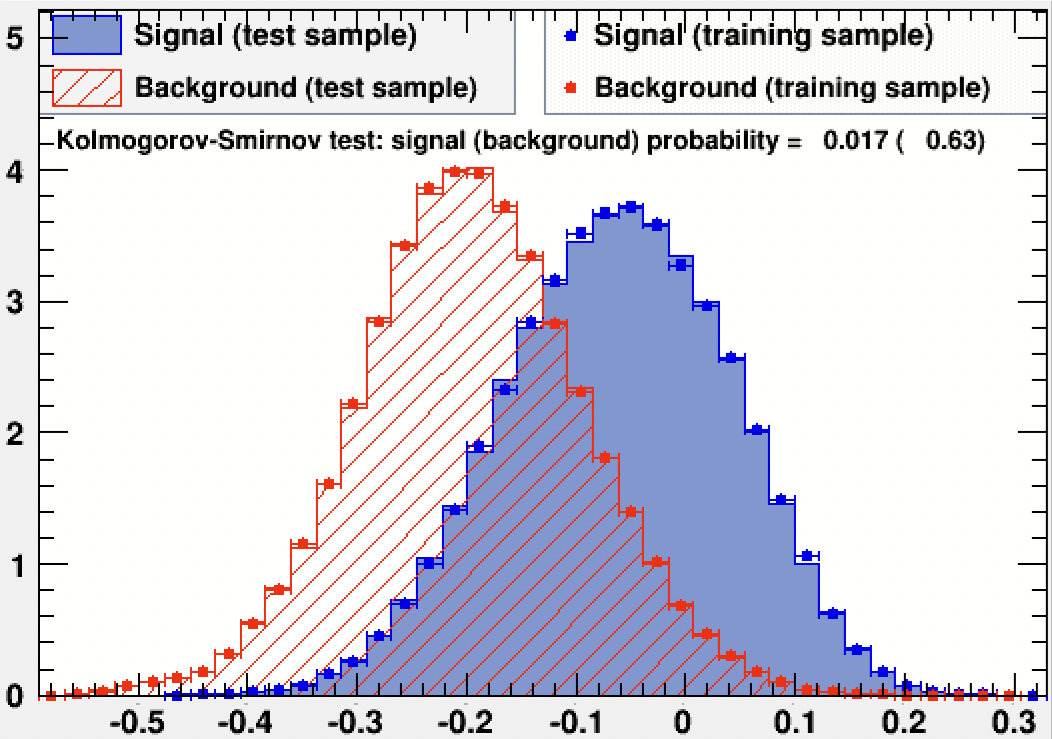
\includegraphics[width=\textwidth]{Analysis/qqh/BDT.png}
  \end{minipage}
}
\subfigure[]
{
  \begin{minipage}[b]{0.42\textwidth}
  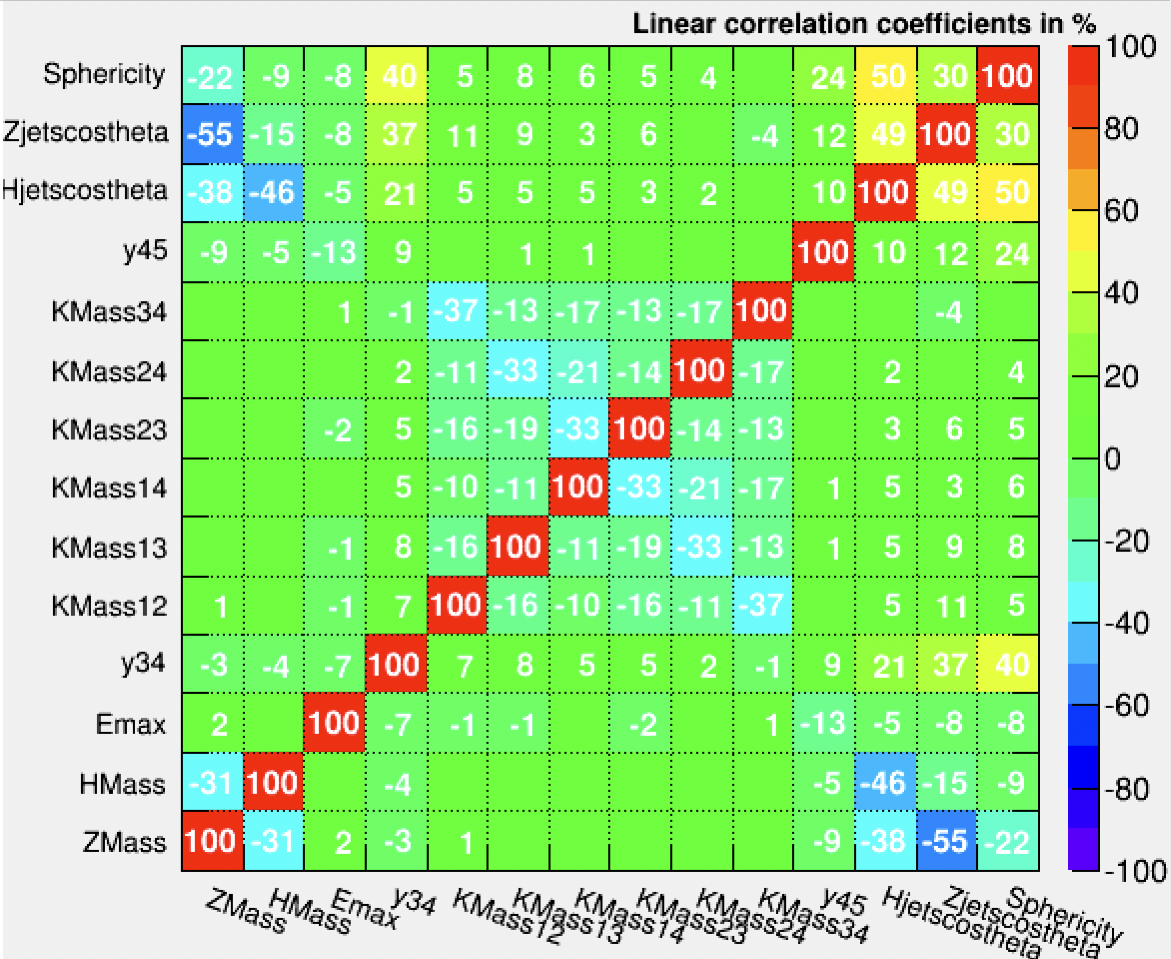
\includegraphics[width=\textwidth]{Analysis/qqh/Correlation.png}
  \end{minipage}
}
\caption{Linear correlation map of variables used in BDT training(left) and the outcome BDT 
response of signal and backgrounds.}
\end{figure}


\begin{table}[!htpb]
\centering
\chuhao
\begin{tabular}{c|c|c|c|c|c|c|c|c|c}\hline
         & \tabincell{c}{signal \\ combined}   &  $\Hboson \to \bpair$   & $\Hboson\to\cpair$   & $\Hboson\to\gpair$   & \tabincell{c}{background\\ combined} & \tabincell{c}{higgs \\background}   &   \tabincell{c}{4 fermions\\ hadronic}&  quark pair &  \tabincell{c}{4 fermion\\ semi-leptonic}  \\ \hline 
 4 jets and iso-lepton veto 
         &  493947 & 413299   & 19362  & 61286  &     75 M      &  299583  &  36.83 M &   23.86M   &   14.72 M      \\ \hline
  $E_{vis} > $206 GeV
         &  459972 &  381470  & 18690  & 59812  &     50.6 M    &  109529  &  28.19 M  &  20.37M  &  1.967M  \\ \hline
 $y_{34} > 0.007$
         &  393979 &  325137 &   15976  & 52866 & 26.4 M        &   100813 &  21.32 M  &  5.207 M  &  218394 \\ \hline
 $N_{jet,pfo} \ge 9$
         &  371240 &  305982 &   14903  & 50355 & 21.4 M        &    82281 &  18.78 M  & 
2.601 M  &  27487  \\ \hline
 $\Delta \theta > $0.92
         &  318163 &  261808 &   12610  & 43745 & 13.55 M       &    71987 &  12.16 M &  
1.315 M  &  4745   \\ \hline
   $X > 0.21$
         &  236652 &  197510 &    9562  & 29580 & 3.15 M        &    38579 &  2.2 M   &  907188   &  3012   \\ \hline
   $BDT > $-0.19
         &  211281 &  177447 &    8324  & 25510 & 1.52 M        &    32653 &  1.08 M  & 
405567   &  580    \\ \hline   
      
\end{tabular}
\caption{Signal and background yields of cutflow in \qqh analysis, normalized to 5000 \ifb}
\label{tab:cut_qqh}
\end{table}


A yth-value is defined according to the PFOs distribution to suppress the background from di-jet events. 